%\clearpage
\section{Empirical Performance Analysis}\label{sec:experiments}
In this section, we perform an empirical evaluation of {\framework}. In the following, we discuss experimental setup, objective of experiments, and experimental results\footnote{Source code, details on preliminaries, and additional experimental results are in the supplementary material.}. 

\noindent\textbf{Experimental Setup.} We implement a prototype of {\framework} in Python (version $ 3.8 $). In {\framework}, we deploy SAlib library~\cite{Herman2017} to compute FIFs based on global sensitivity analysis. In our experiments, we consider five widely studied datasets in fairness literature, namely COMPAS, Adult, German-credit, Ricci, and Titanic. We deploy Scikit-learn library to learn different classifiers: Logistic Regression, Support Vector Machine, Decision Tree, and \red{Neural Networks}. \red{We set $ \lambda = 2 $ meaning that we allow {\framework} to compute inter-sectional influences up to order two.}

We compare {\framework} with Shapley-valued based FIF computational framework, referred as SHAP. In addition, we deploy {\framework} on different fairness enhancing and fairness attack algorithms and analyze the effect of these algorithms on the FIFs and the resultant fairness metric. In the following, we discuss the objective of our empirical study. 

1. How does {\framework} compare with SHAP in terms of accuracy in computing FIFs and the resulting bias?

2. What is the impact of inter-sectional vs.\ individual FIFs in understanding the sources of bias of a classifer?

3. How do FIFs change while applying different fairness enhancing and fairness attack algorithms?

4. What is the effect of $ \lambda $ on the runtime of {\framework}?

In summary...

%\subsection{Experimental Results}
%In the following we discuss our experimental results in detail. 


%\clearpage
\begin{figure}
	\centering
	\subfloat{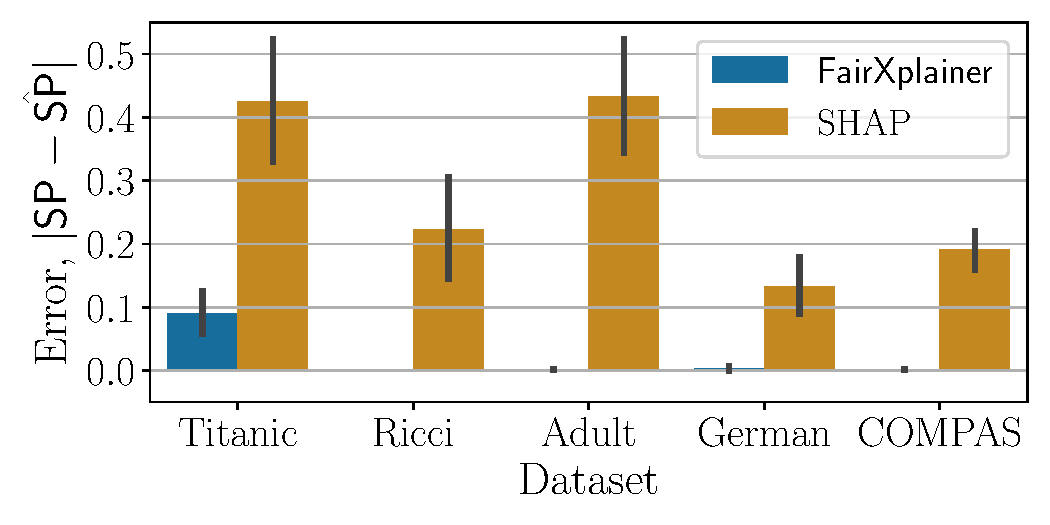
\includegraphics[scale=0.4]{figures/sp_train_accuracy}}
	\subfloat{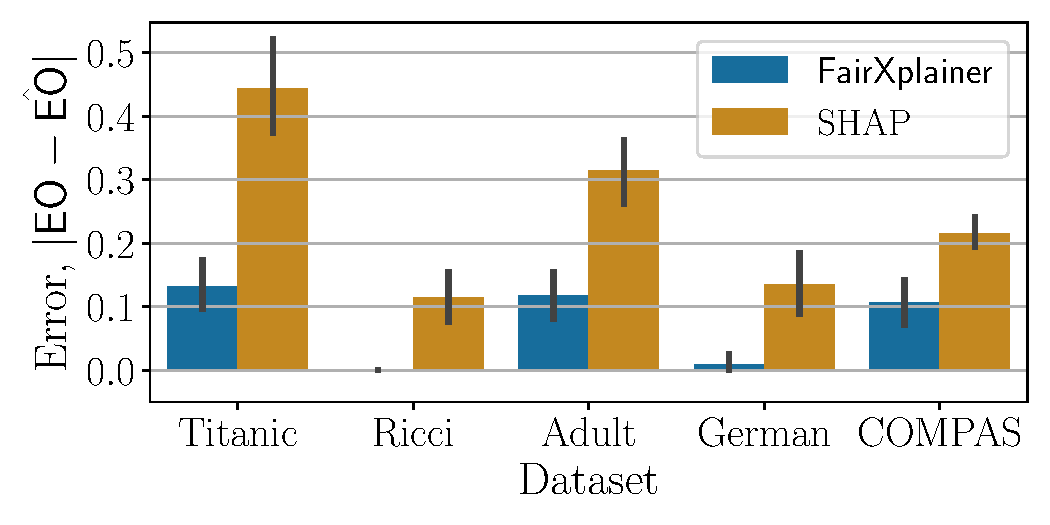
\includegraphics[scale=0.4]{figures/eo_train_accuracy}}
	%	\subfloat[]{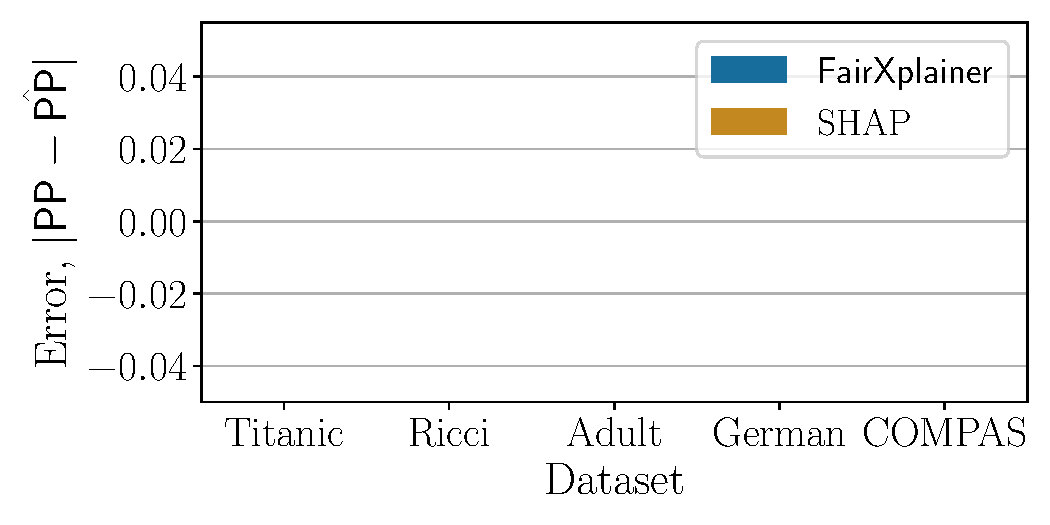
\includegraphics[scale=0.3]{figures/suff_train_accuracy}}\\
	%	\subfloat[]{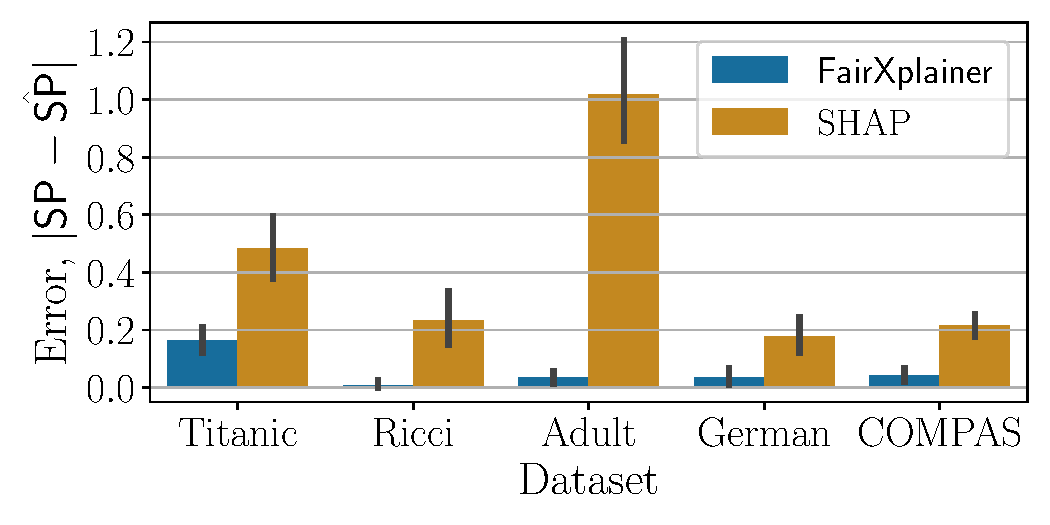
\includegraphics[scale=0.3]{figures/sp_test_accuracy}}
	%	\subfloat[]{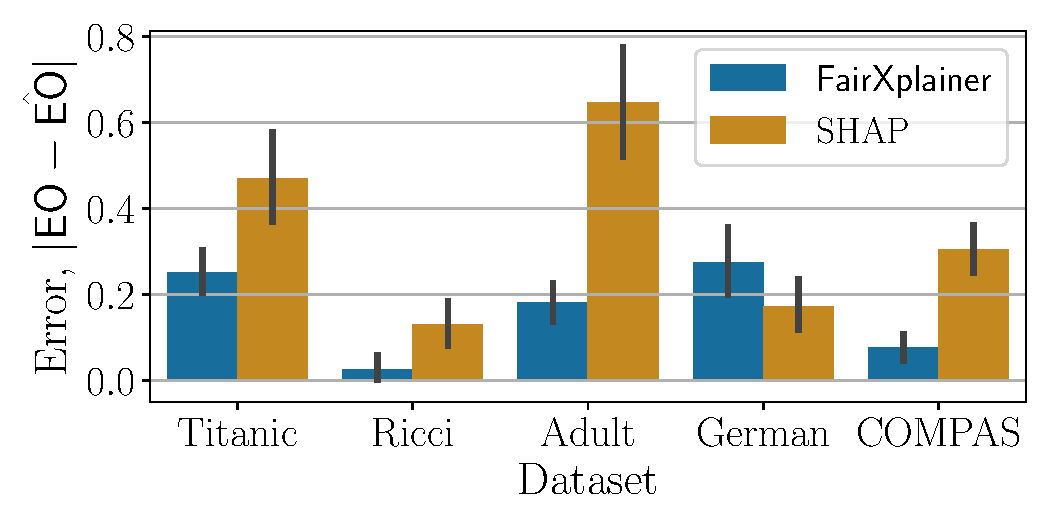
\includegraphics[scale=0.3]{figures/eo_test_accuracy}}
	%	\subfloat[]{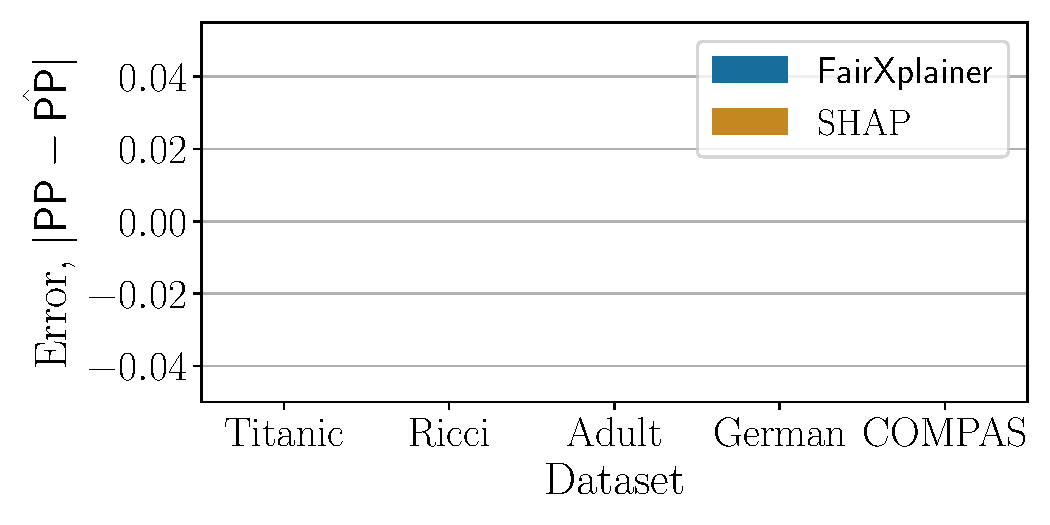
\includegraphics[scale=0.3]{figures/suff_test_accuracy}}\\
	
	\caption{Comparison between {\framework} and SHAP on estimation error of fairness metrics. Lower values on the $ Y $-axis denote a better result. \red{Add results for EO and CUAE}}
	\label{fig:estimation_error}
\end{figure}


\paragraph{Estimation Error of Bias.} We compare {\framework} with SHAP in estimating statistical parity $ \mathsf{SP} $ and equalized odds $ \mathsf{EO} $, where each metric is calculated by summing all FIFs (Axiom~\ref{axm:additivity}). We consider \red{five} datasets, each trained on \red{three} different classifiers by applying five fold cross-validation. We compute estimation error by taking the absolute difference between the exact and  estimated value of a metric and present results in Figure~\ref{fig:estimation_error}. In both metrics, {\framework} demonstrates significantly less estimation error than SHAP. For example, the mean error of {\framework} in estimating $ \mathsf{SP} $ on Titanic dataset is $ 0.1 $ vs $ 0.42 $ for SHAP. In this context, the estimation error of {\framework} is due to the degenerate cases in Section~\ref{sec:fifs}, where $ \Pr[\hat{Y} = 1 | \sensitive = \mathbf{a}] $ is either $ 1 $ or $ 0 $.  Therefore, local explanation based approach SHAP is significantly inaccurate in computing FIFs and corresponding fairness metric than global sensitivity analysis based approach {\framework}.


\begin{figure}
	\centering
	\subfloat[Individual FIFs]{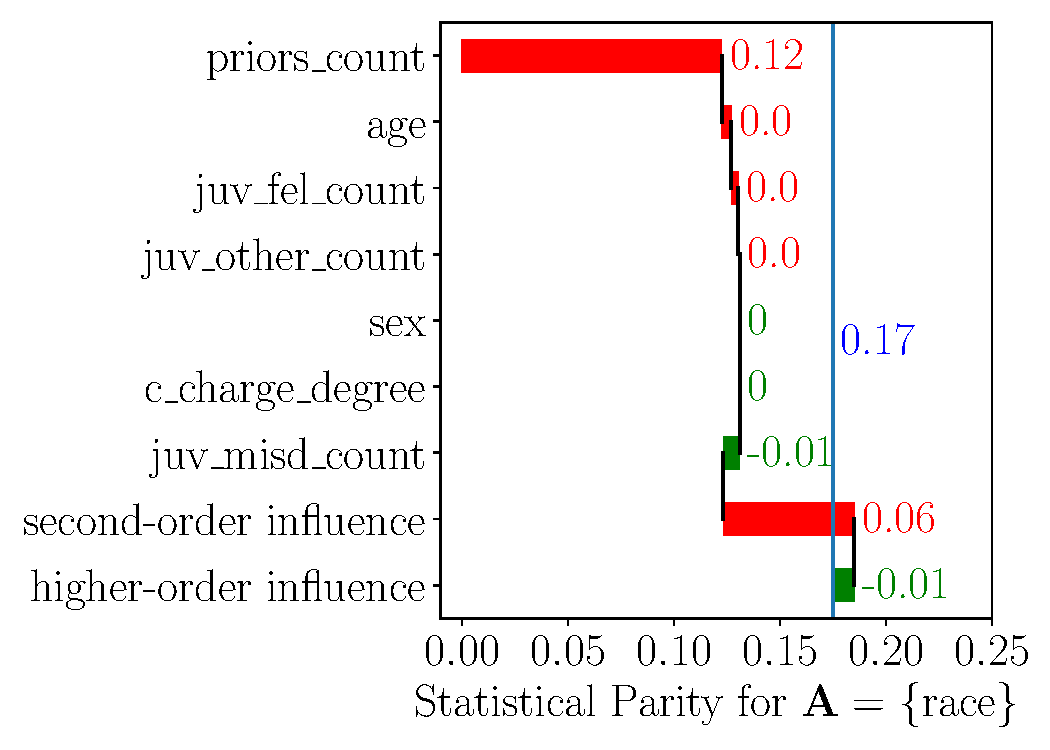
\includegraphics[scale=0.35]{figures/feature_weight_unsorted}\label{fig:individual_fifs}}
	\subfloat[Individual and intersectional FIFs]{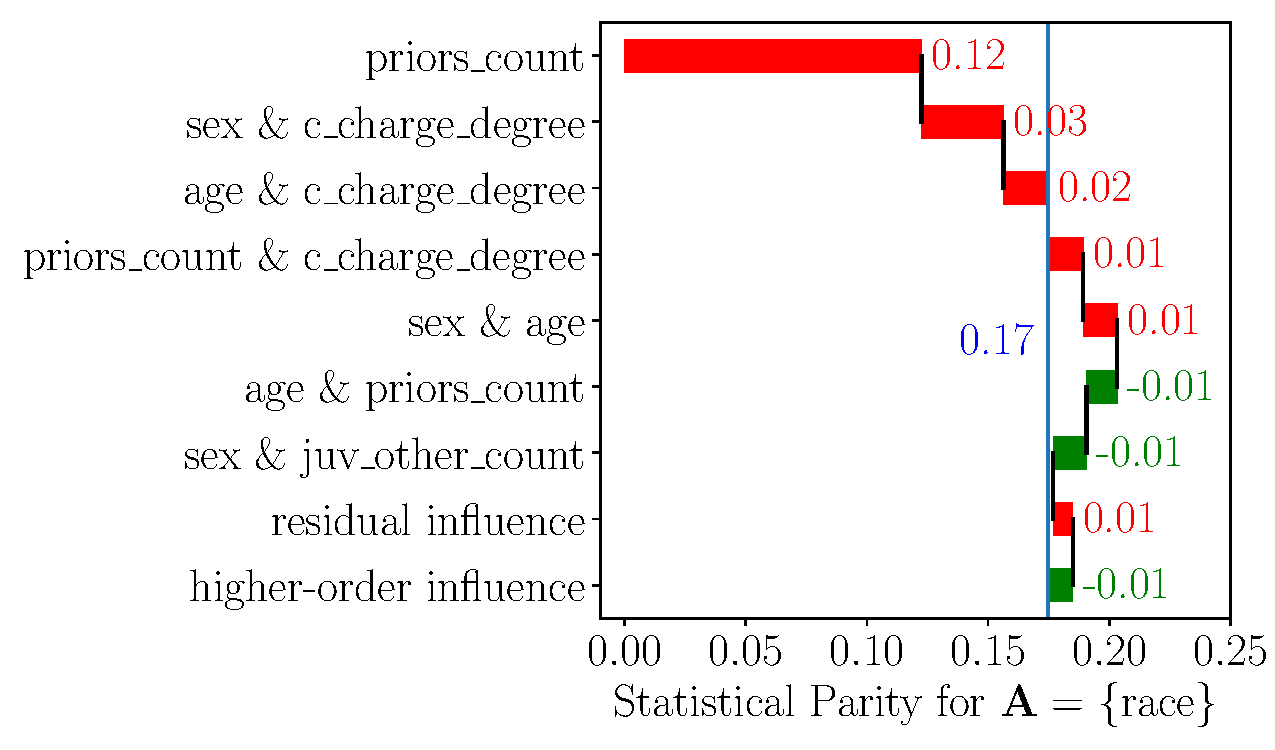
\includegraphics[scale=0.35]{figures/feature_weight}\label{fig:individual_and_intersectional_fifs}}\\
	\caption{Explaining statistical parity in COMPAS dataset for the sensitive feature `race' using HDMR method. \red{Effect to be influence. Change 'Feature' from Y axis. SP in different color and in the title. X axis label = statistical parity w.r.t.\ race. An experiment comparing LR and NN (showing accuracy, sp and FIFs side by side.)}}
	\label{fig:individual_vs_intersectional_influence}
\end{figure}



\paragraph{Individual vs.\ Inter-sectional FIFs.} Our first experiment is to understand the importance of inter-sectional FIFs over individual FIFs. We consider COMPAS dataset with race = \{Caucasian, non-Caucasian\} as the sensitive feature and a logistic regression classifier to predict whether a person will re-offend crimes within the next two years. Since the classifier only optimizes training error, it demonstrates statistical parity as $ 0.17 $, denoting that a non-Caucasian  has $ 0.17 $ higher probability of re-offending crimes than a Caucasian. Next, we investigate the source of bias and present individual FIFs in Figure~\ref{fig:individual_fifs} and both individual and intersectional FIFs in Figure~\ref{fig:individual_and_intersectional_fifs}. In both figures, we show top seven influential FIFs sorted by absolute values, followed by residual high-order FIFs. In Figure~\ref{fig:individual_fifs}, `priors count' of an individual is dominating in increasing statistical parity (FIF $ = 0.12 $). Other non-sensitive features appear to have almost zero FIFs. However, the sum of second-order influences of all features increases statistical parity by $ 0.06 $, denoting that the data is highly correlated and presenting only individual FIFs does not demonstrate the true sources of bias. For example, while both `sex' and `age' of persons have zero influence on bias in an individual level (Figure~\ref{fig:individual_fifs}), these features together with `c charge degree', `priors count', and `juvenile other count' contribute highly on statistical parity (sum of FIF $ = 0.03 + 0.02 + 0.01 + 0.01 - 0.01 - 0.01 = 0.05$). Therefore, inter-sectional influences together with individual influences demonstrate a clear understanding on the source of bias of a classifier. Note that, unlike SHAP, {\framework} is the only framework to compute beyond individual FIFs.








%\clearpage

\begin{figure}
	\centering
	\subfloat{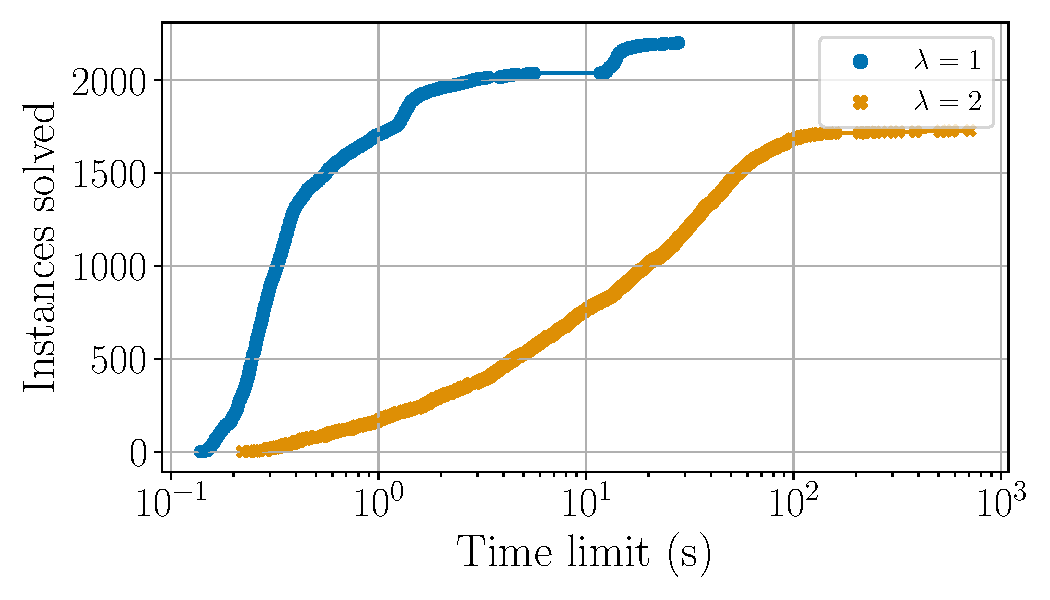
\includegraphics[scale=0.4]{figures/vary_max_order_train}}
%	\subfloat[]{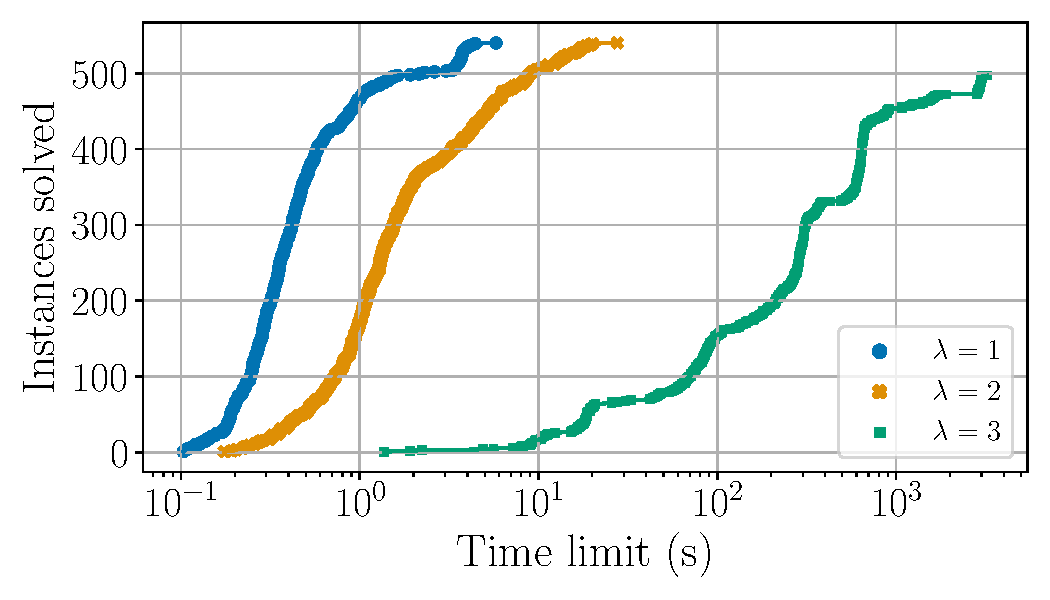
\includegraphics[scale=0.4]{figures/vary_max_order_test}}	
	\caption{Varying max-order $ \lambda $.}
	\label{fig:varying_max_order}
\end{figure}

\paragraph{Effect of Max-order $ \lambda $.} We experiment the effect of \red{$ \lambda \in \{1, 2, 3\} $} on the runtime of {\framework}. For each $ \lambda $, \blue{we consider $ 1086 $ fairness instances ($ 5 $ datasets totaling to $ 27 $ different combinations of sensitive features $ \times $ $ 5 $-fold cross validation $ \times $ $ 8 $ classifiers)}. In the \red{cumulative plot} in  Figure~\ref{fig:varying_max_order}, $ X $-axis denotes runtime and $ Y $-axis denotes total solved instances; a point $ (x,y) $ denotes that $ y $ many instances are solved within $ x $ seconds. As we increase $ \lambda $, {\framework} requires more time (around $ 0.5 $ order of magnitude) to solve equal number of instances. Because, for higher $ \lambda $, there is a combinatorial explosion in the number of component functions in the backfitting algorithm. Thus, an computing higher-order FIFs results in a higher runtime of {\framework}.



\begin{comment}
TODO
\begin{itemize}
	\item all group fairness metrics
	\item vary sample size  and dimension of features (add statistics for each dataset in the figure)
	\item runtime vs max-order $ \lambda $
	\item draw $ 1/n $, $ 1/n^{1/2} $, $ 1/n^{1/3} $, std.
	\item \red{Experiment of fairness enhancing and attack algo on the same dataset.} 
\end{itemize}
\end{comment}



\section{Conclusion}
In this paper, we propose {\fvgm}, an efficient fairness verification framework for linear classifiers based on a novel stochastic subset-sum problem. {\fvgm} encodes a graphical model of feature-correlations, represented as a Bayesian Network, and computes multiple group and causal fairness metrics accurately. We experimentally demonstrate that {\fvgm} is not only more accurate and scalable than the existing verifiers but also applicable in practical fairness tasks, such as verifying fairness attacks and enhancing algorithms, and computing the fairness influence functions. 
As a future work, we aim to design fairness-enhancing algorithms certified by fairness verifiers, such as {\fvgm}. %We also investigate a principled approach to detect the sources of bias by computing fairness influence functions (FIF). 
Since {\fvgm} serves as an accurate and scalable fairness verifier for linear classifiers, it will be interesting to design such verifiers for other ML models.





\clearpage


\begin{figure}
	\centering
	\subfloat[]{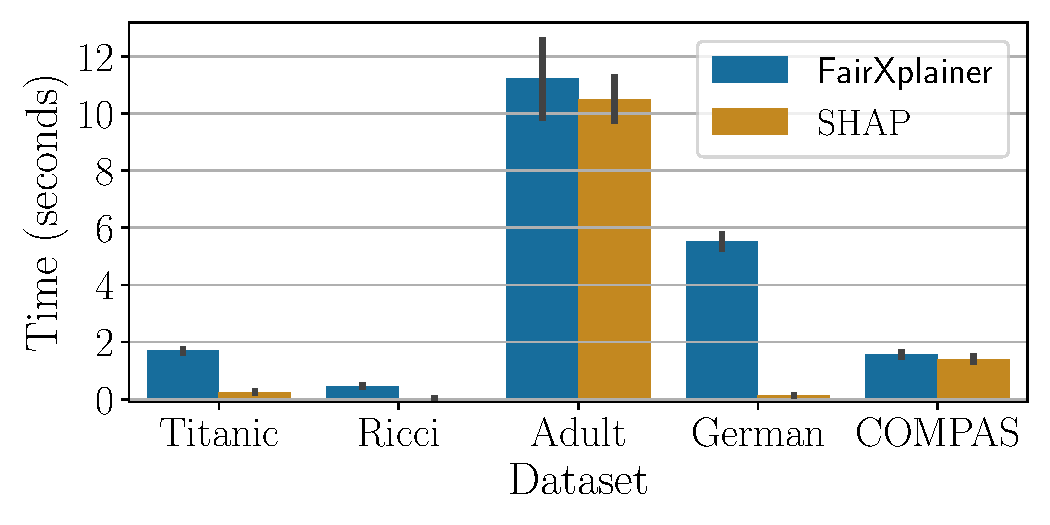
\includegraphics[scale=0.3]{figures/sp_train_time}}
	\subfloat[]{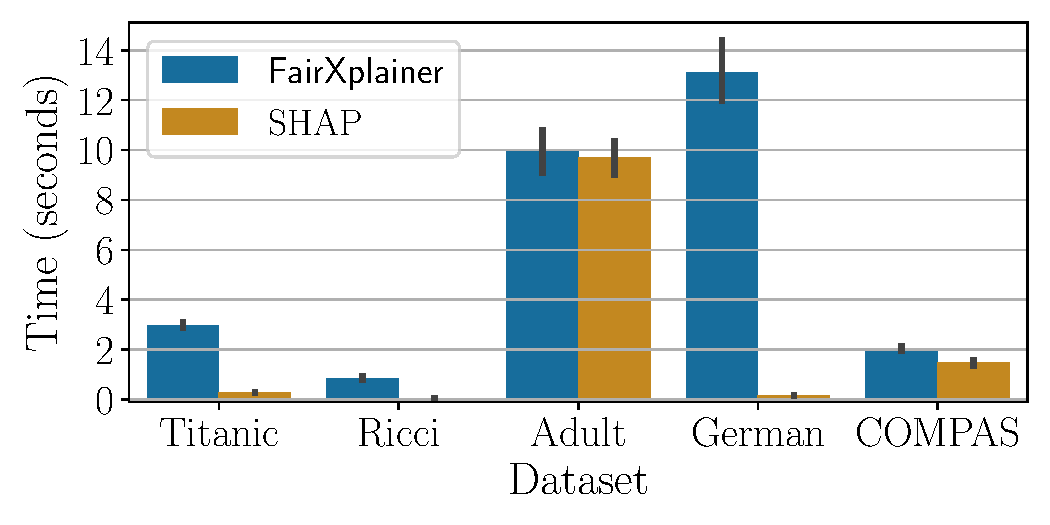
\includegraphics[scale=0.3]{figures/eo_train_time}}
	\subfloat[]{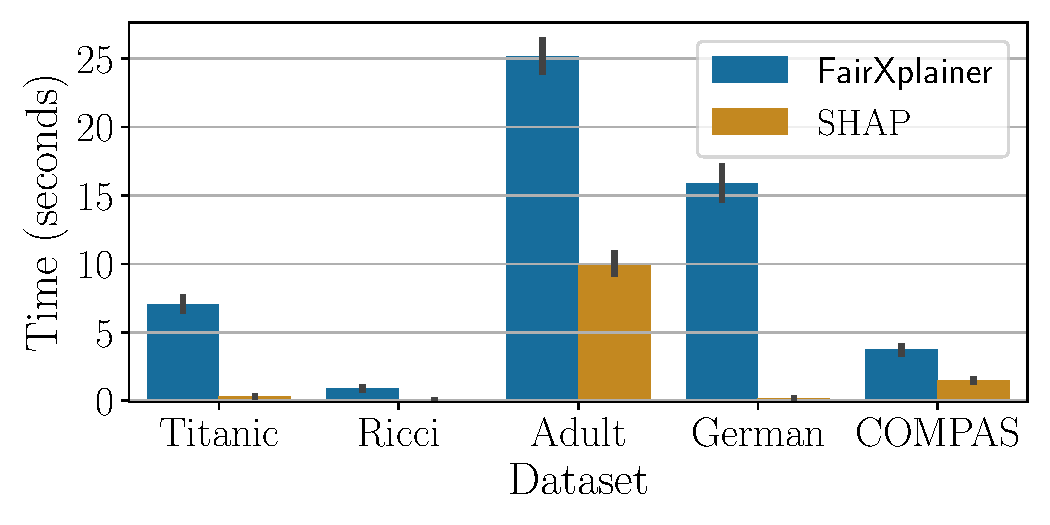
\includegraphics[scale=0.3]{figures/suff_train_time}}\\
	\subfloat[]{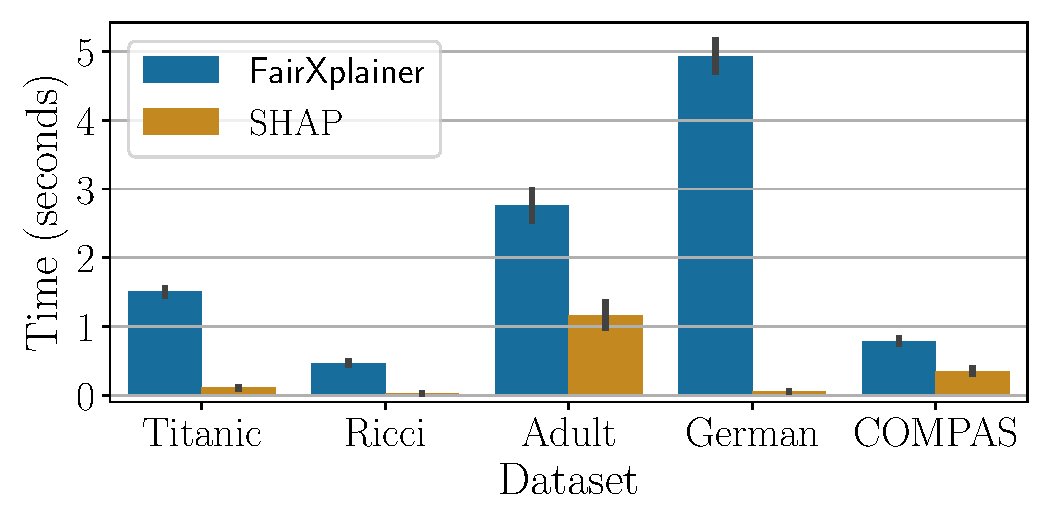
\includegraphics[scale=0.3]{figures/sp_test_time}}
	\subfloat[]{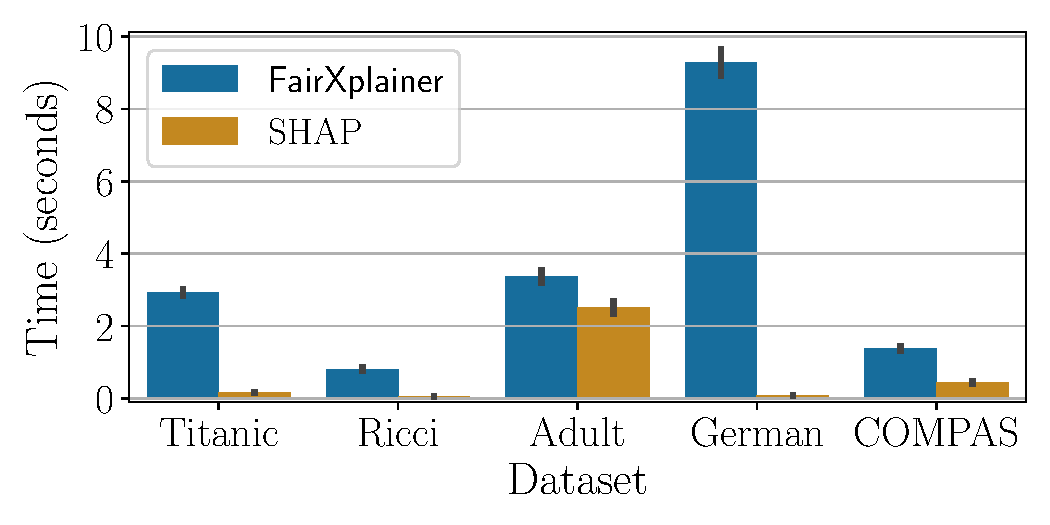
\includegraphics[scale=0.3]{figures/eo_test_time}}
	\subfloat[]{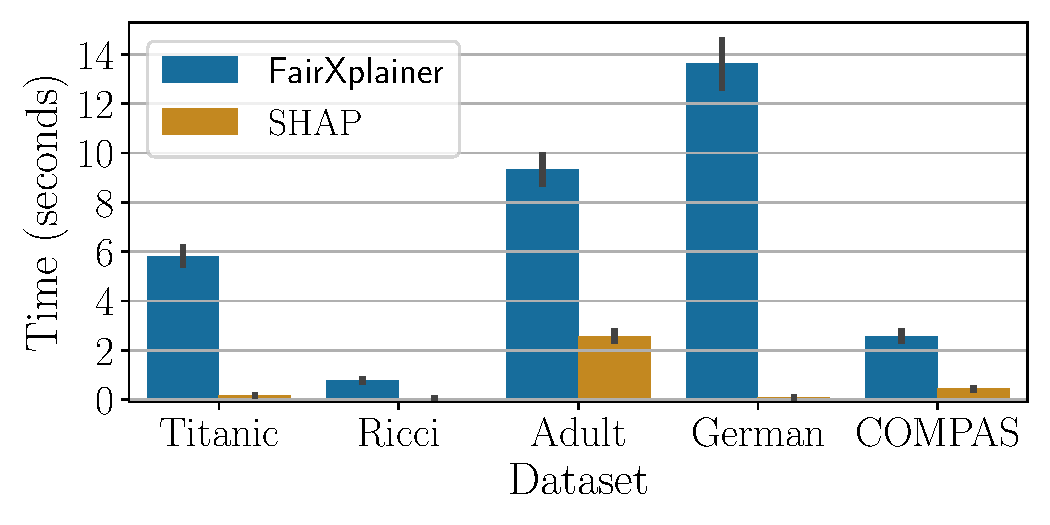
\includegraphics[scale=0.3]{figures/suff_test_time}}\\
	\caption{Comparison between {\framework} and SHAP on runtime. Lower values on the $ Y $-axis are better. \red{[Should be discussed in the Supplementary material.]}}
\end{figure}





\begin{figure}
	\centering
	\subfloat[Unsorted weights]{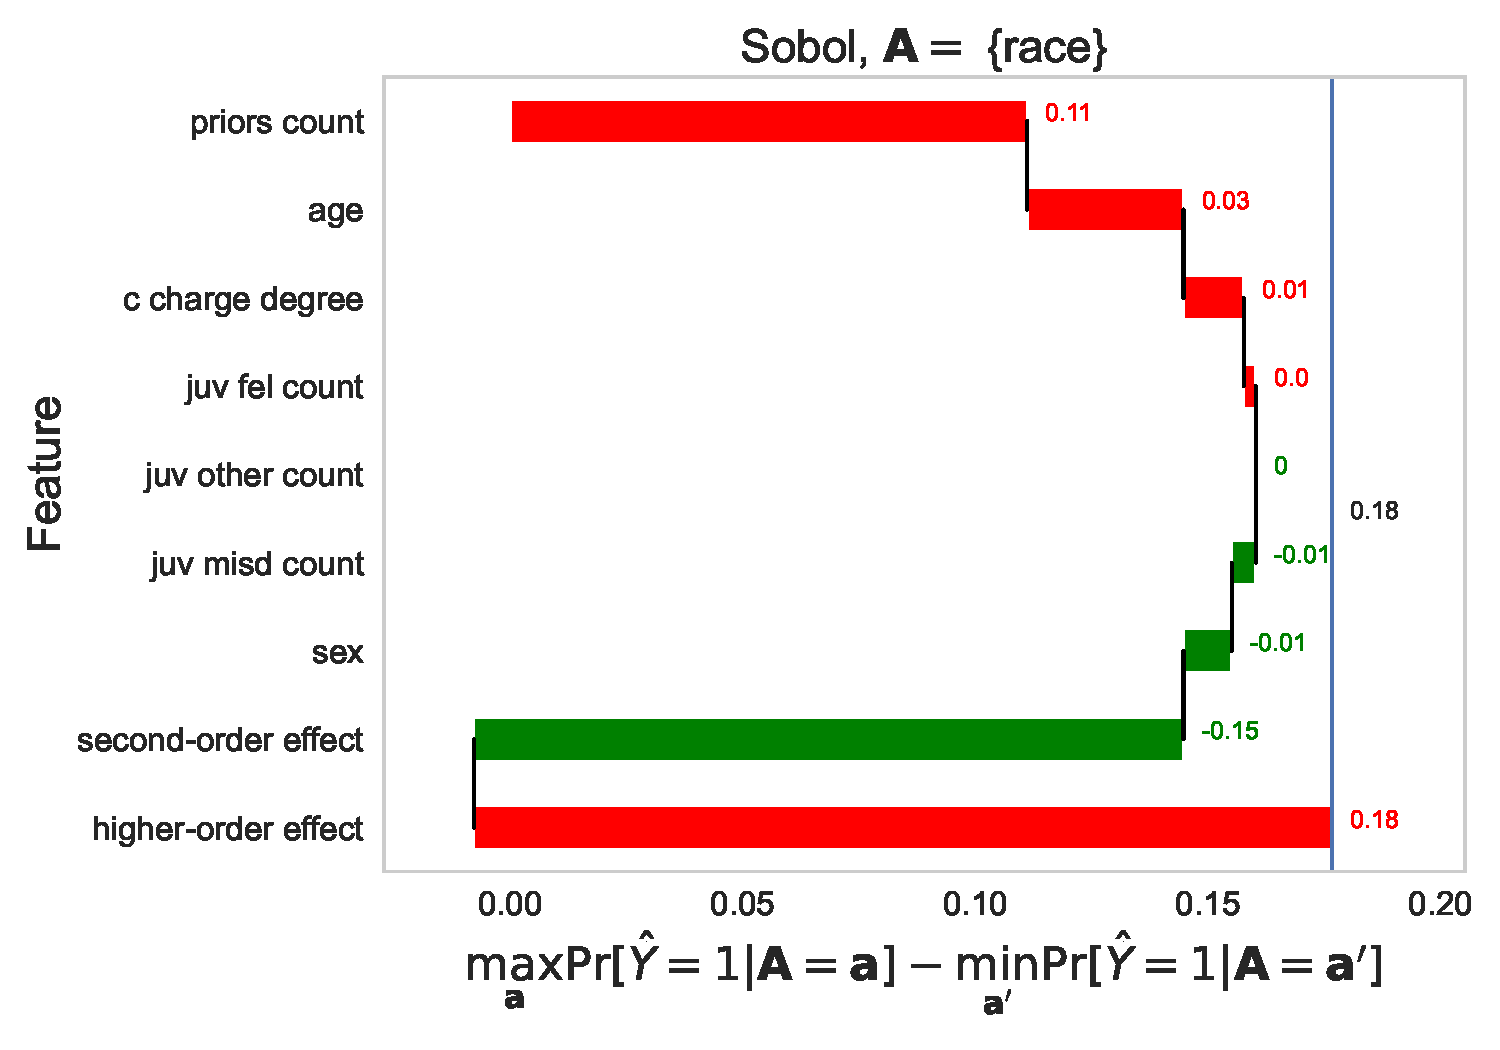
\includegraphics[scale=0.45]{figures/feature_weight_sobol_unsorted}}\\
	\subfloat[Sorted weights including first and second order effect]{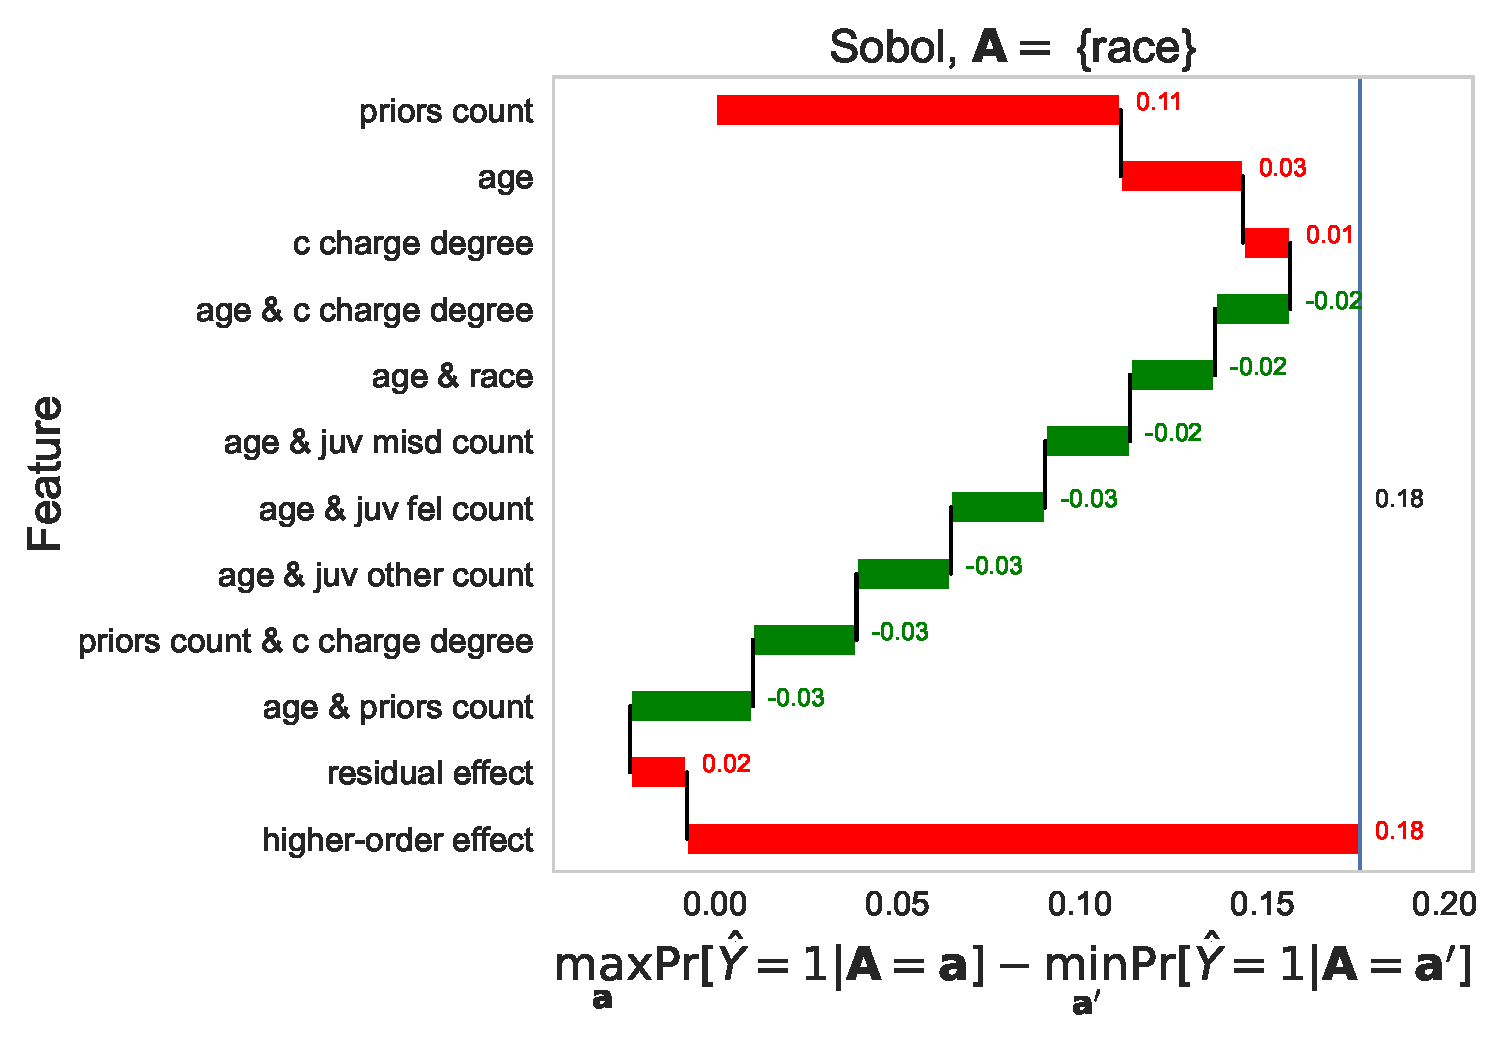
\includegraphics[scale=0.45]{figures/feature_weight_sobol}}\\
	\caption{Explaining statistical parity in COMPAS dataset for the sensitive feature `race' using Sobol method. This approach takes the (independent) distribution of features as input instead of a dataset. We apply KDE (Kernel Density Estimation) to learn the PDF of each feature.}
\end{figure}


\begin{figure}
	\centering
	\subfloat{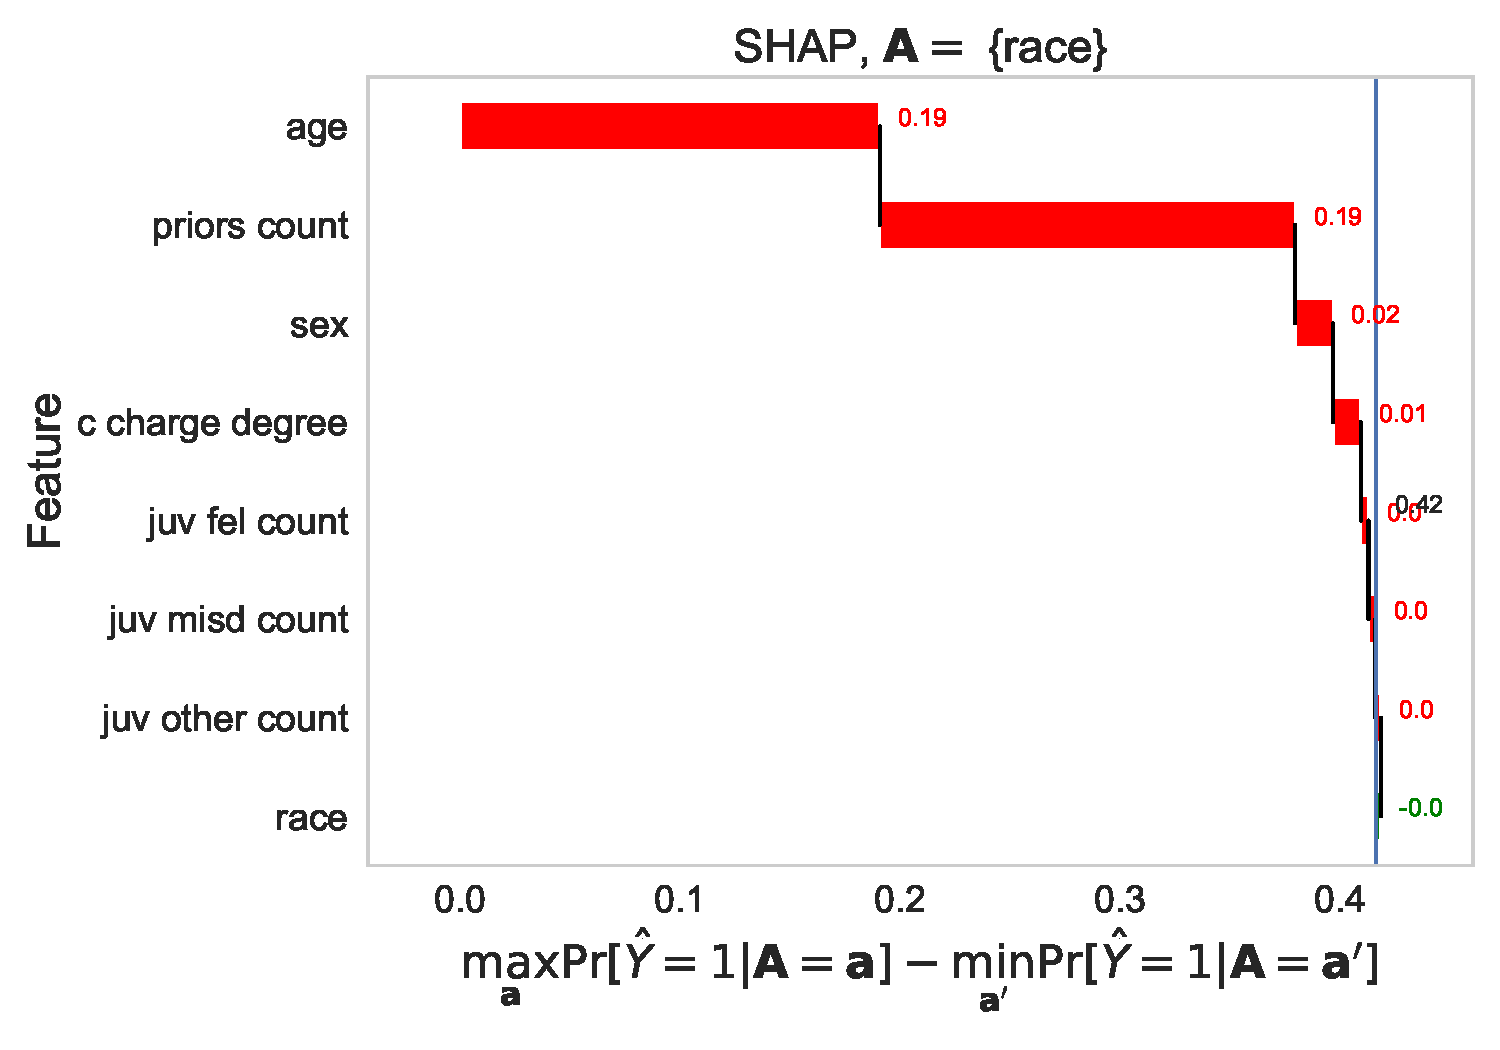
\includegraphics[scale=0.45]{figures/feature_weight_shap}}\\
	\caption{Explaining statistical parity in COMPAS dataset for the sensitive feature `race' using Shap method. This method is based on local explanations of classifiers. We observe higher discrepancy of this explanation as the computed statistical parity is often far from the exact value. Shap method can explain effect of individual features, which is a crucial limitation.}
\end{figure}

\begin{figure}
	\centering
	\subfloat{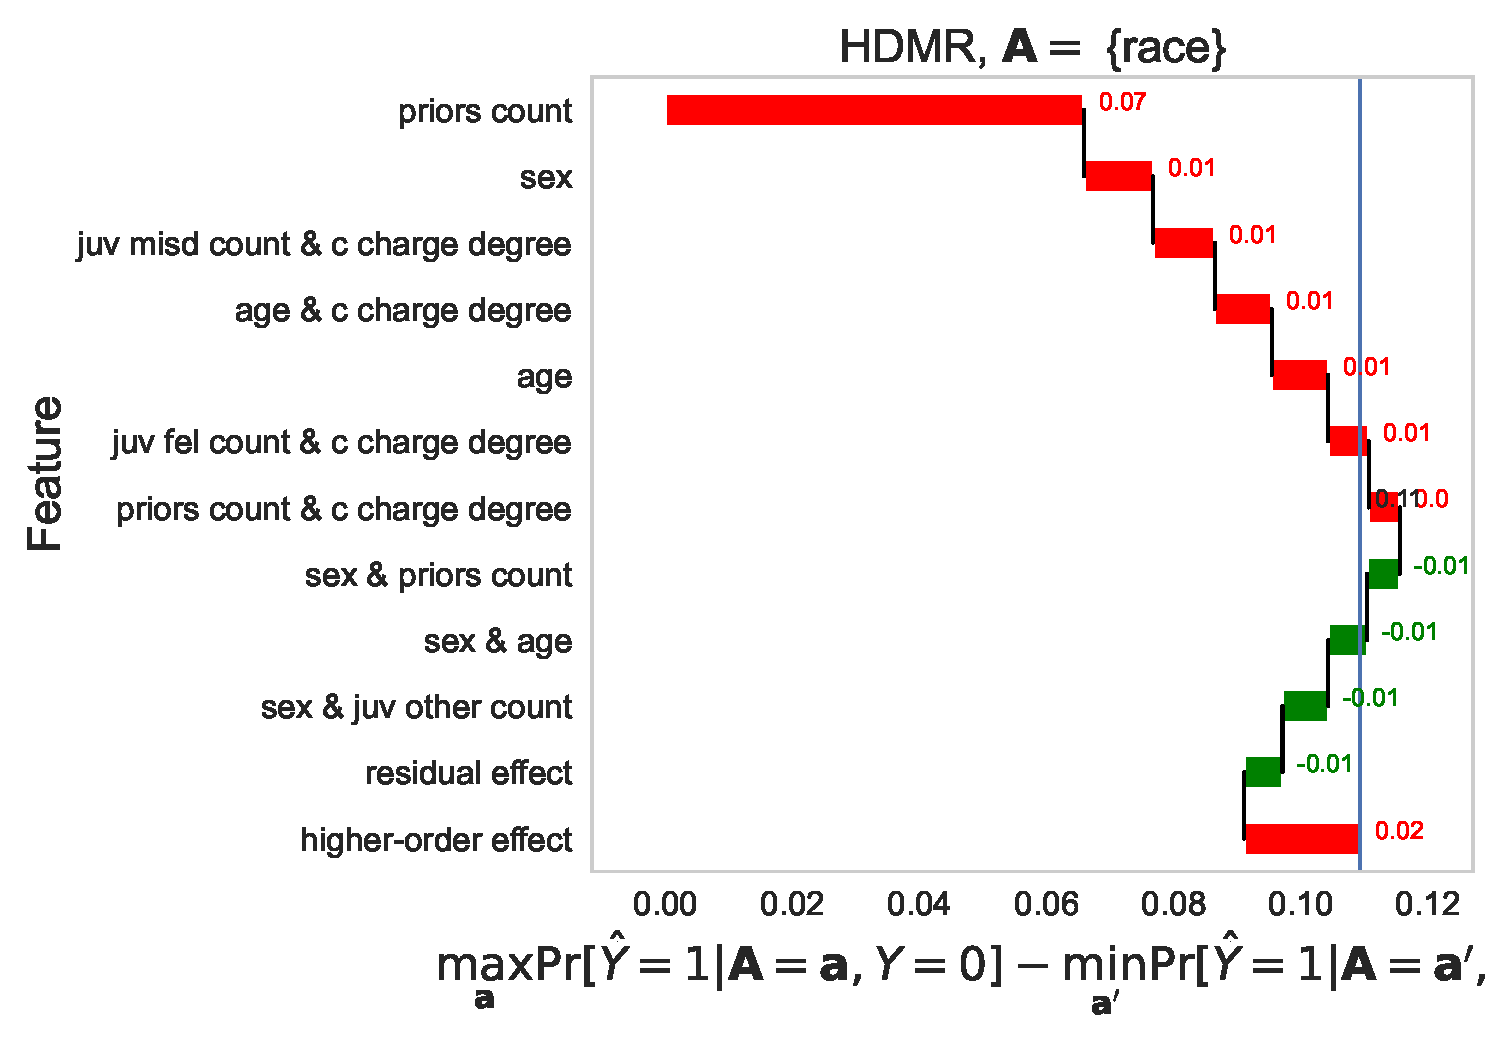
\includegraphics[scale=0.45]{figures/feature_weight_eo_y_0}}\\
	\subfloat{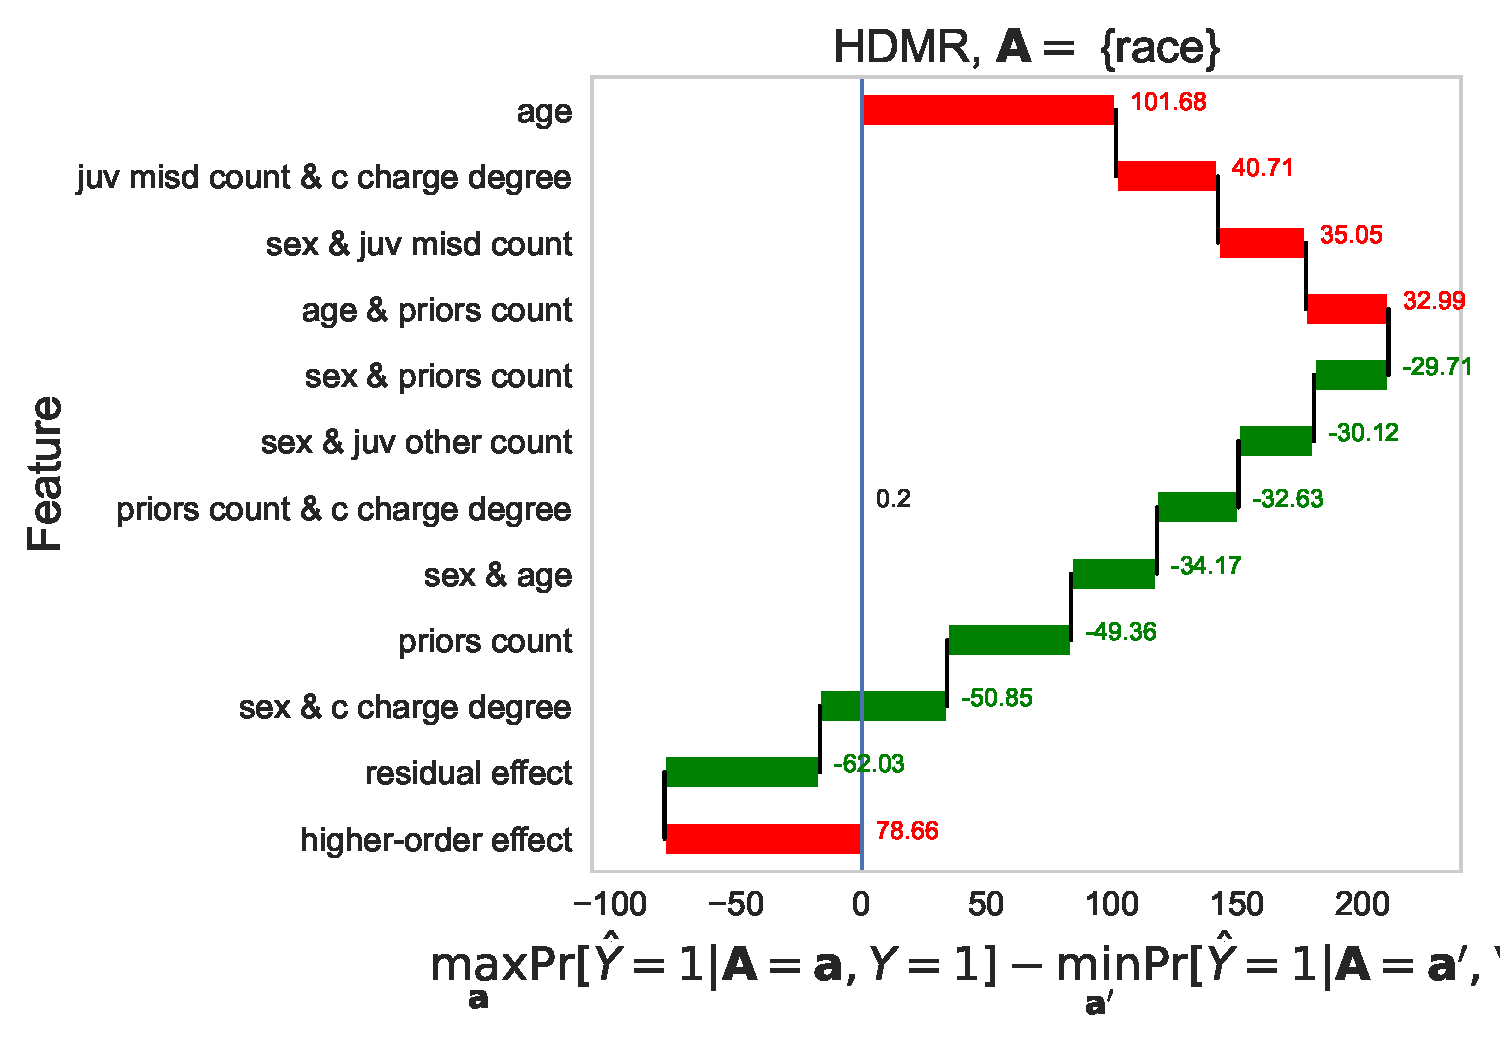
\includegraphics[scale=0.45]{figures/feature_weight_eo_y_1}}\\
	\caption{Explaining equalized odds in COMPAS dataset for the sensitive feature `race' using HDMR method.}
\end{figure}


\begin{figure}
	\centering
	\subfloat{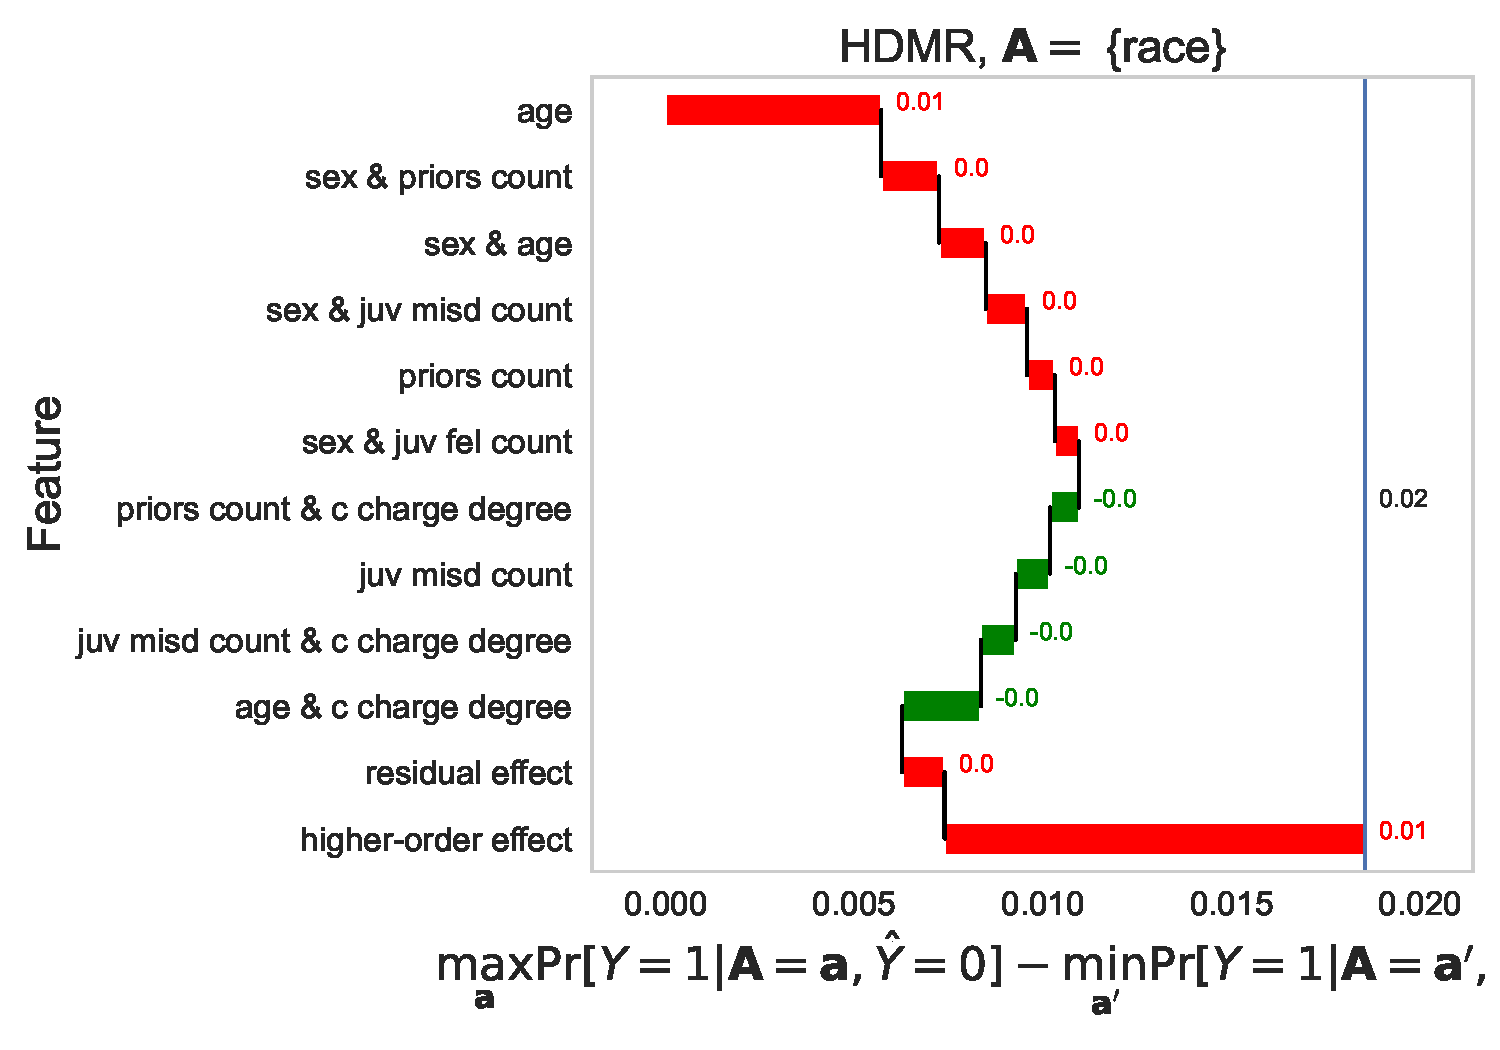
\includegraphics[scale=0.45]{figures/feature_weight_sufficiency_y_0}}\\
	\subfloat{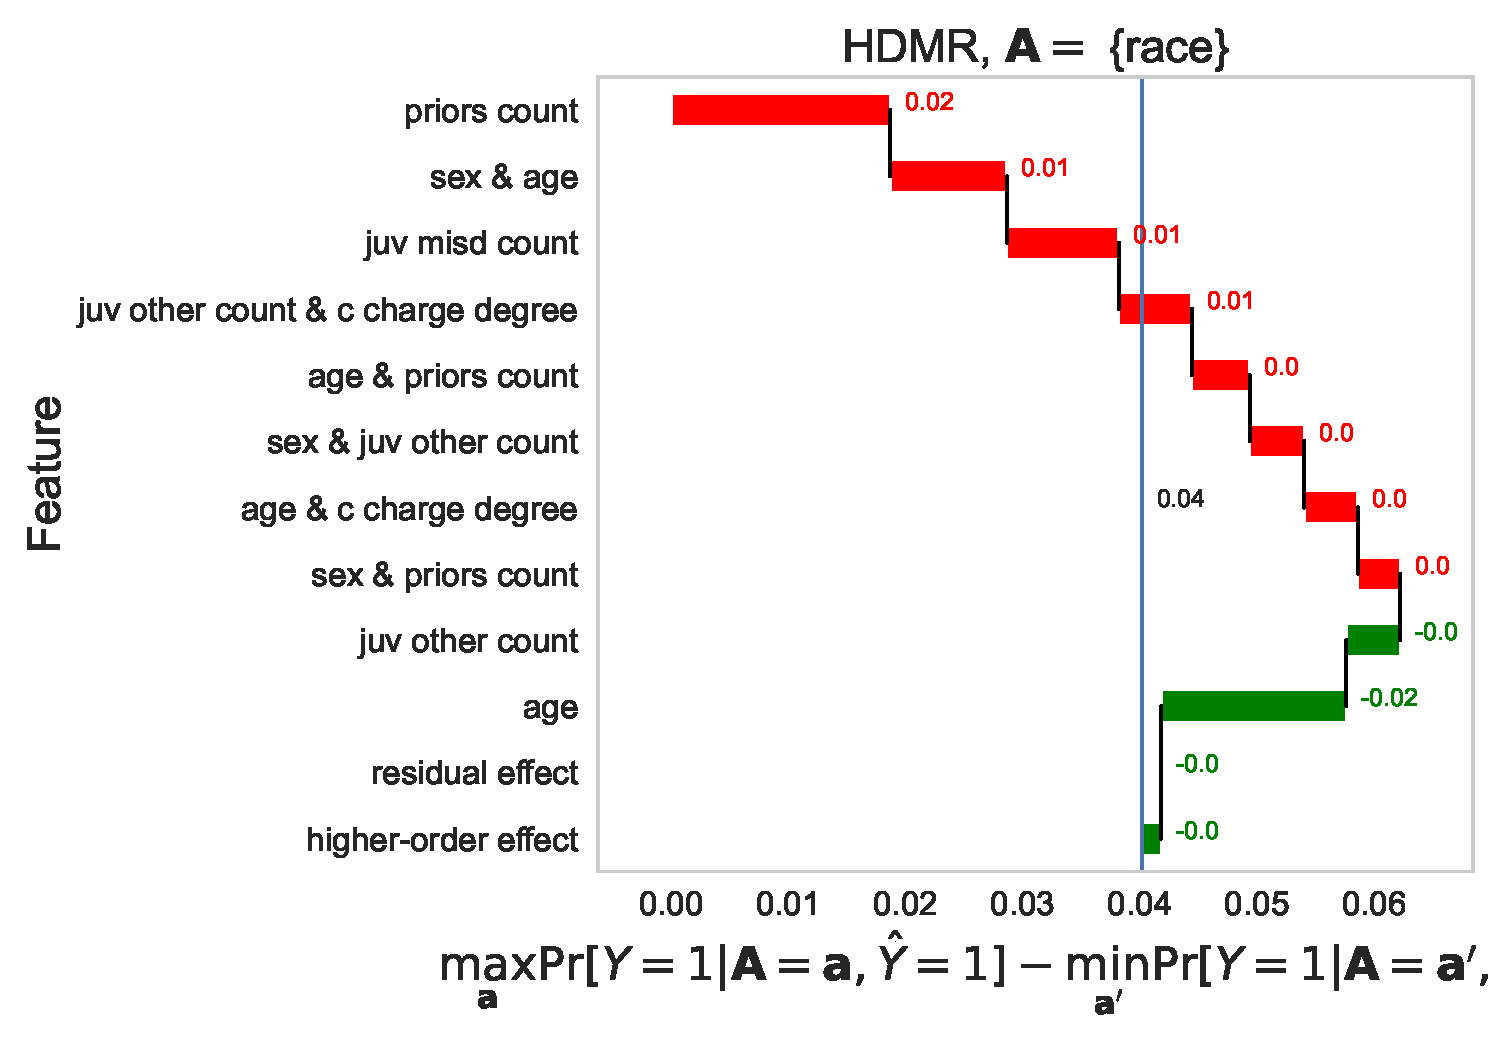
\includegraphics[scale=0.45]{figures/feature_weight_sufficiency_y_1}}\\
	\caption{Explaining sufficiency fairness metrics in COMPAS dataset for the sensitive feature `race' using HDMR method.}
\end{figure}


\begin{figure}
	\centering
	\subfloat{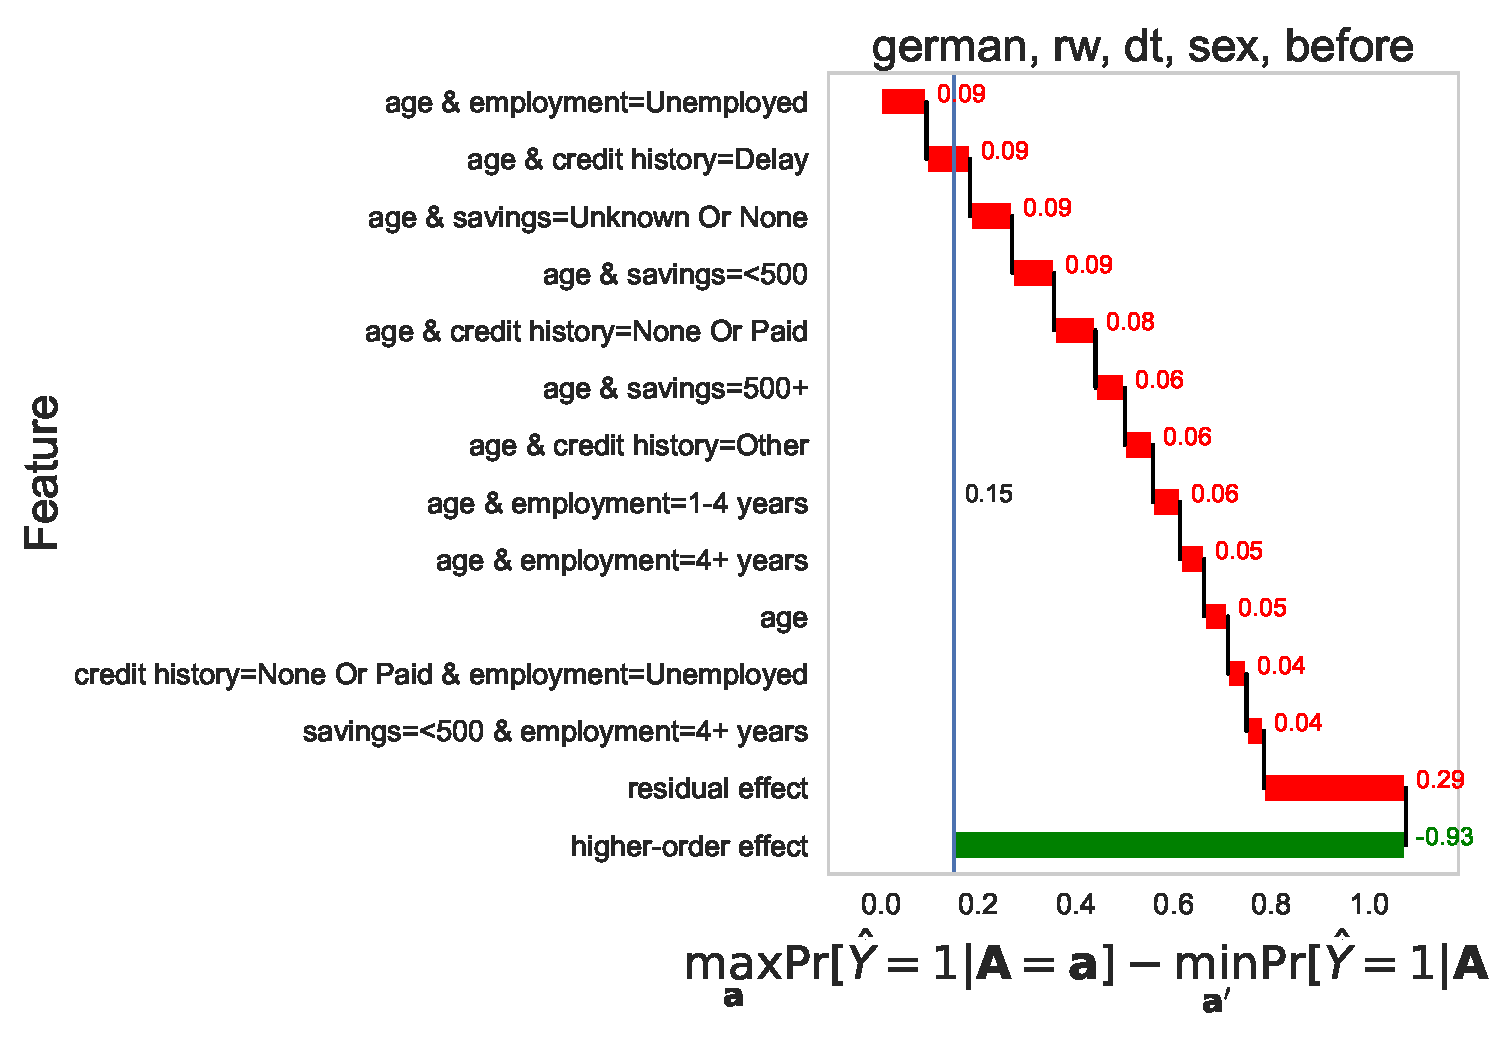
\includegraphics[scale=0.45]{figures/german_rw_dt_sex_before}}\\
	\subfloat{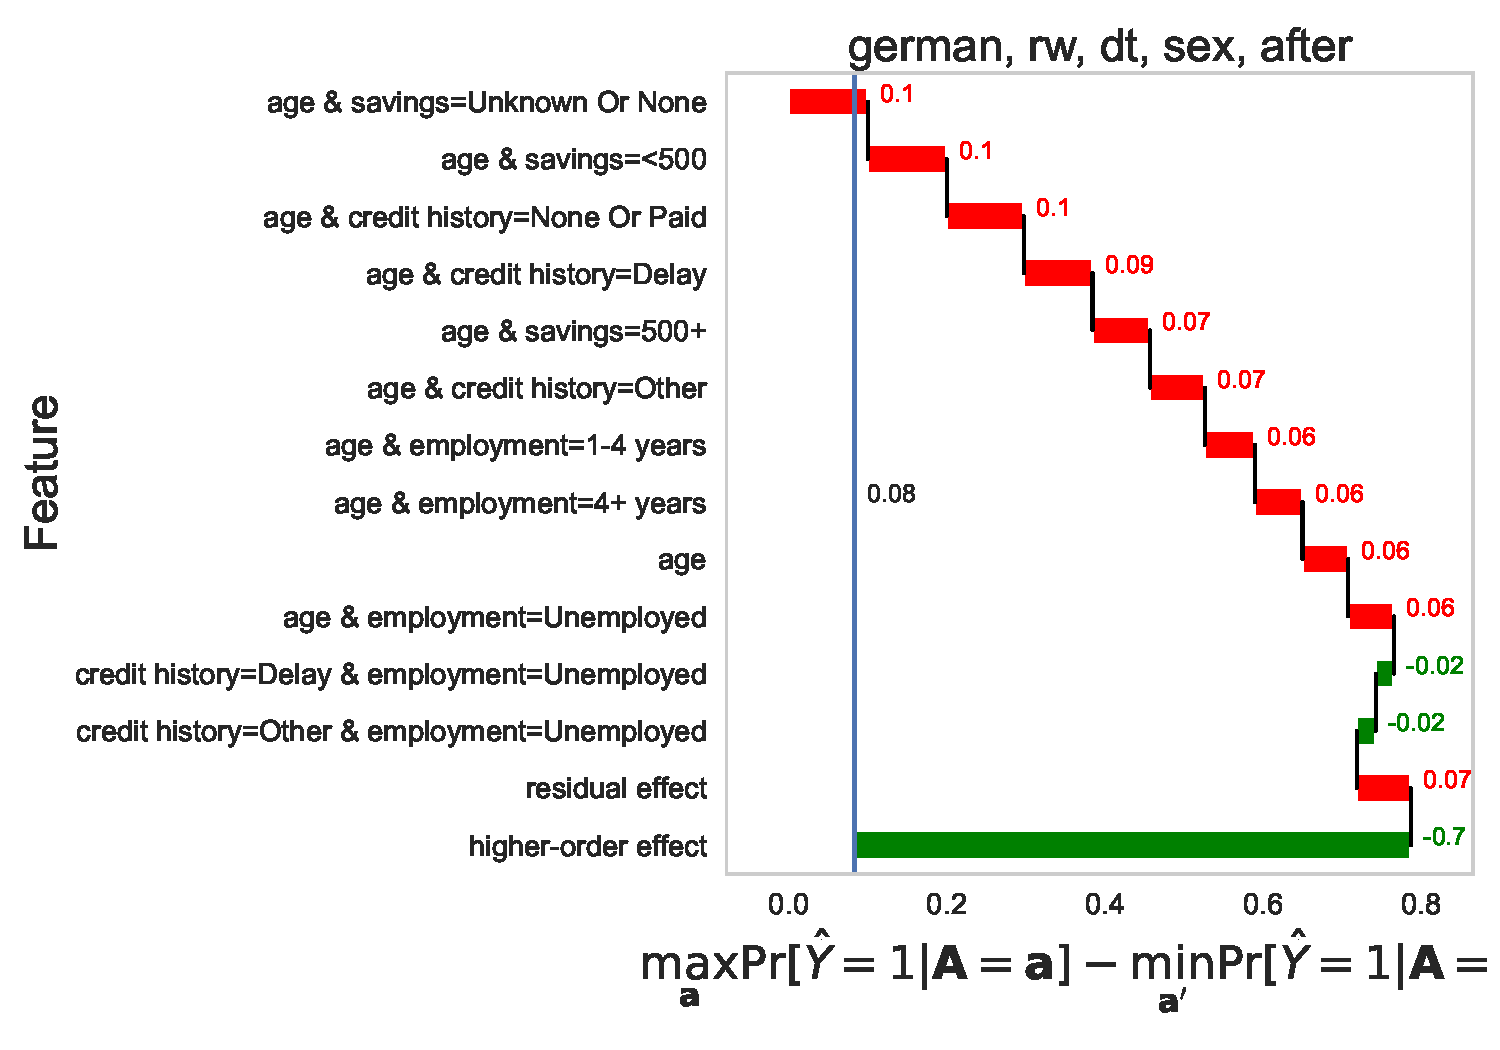
\includegraphics[scale=0.45]{figures/german_rw_dt_sex_after}}
	\caption{Fairness enhancing preprocessing algorithm, reweighing..}
\end{figure}

\begin{figure}
	\centering
	\subfloat{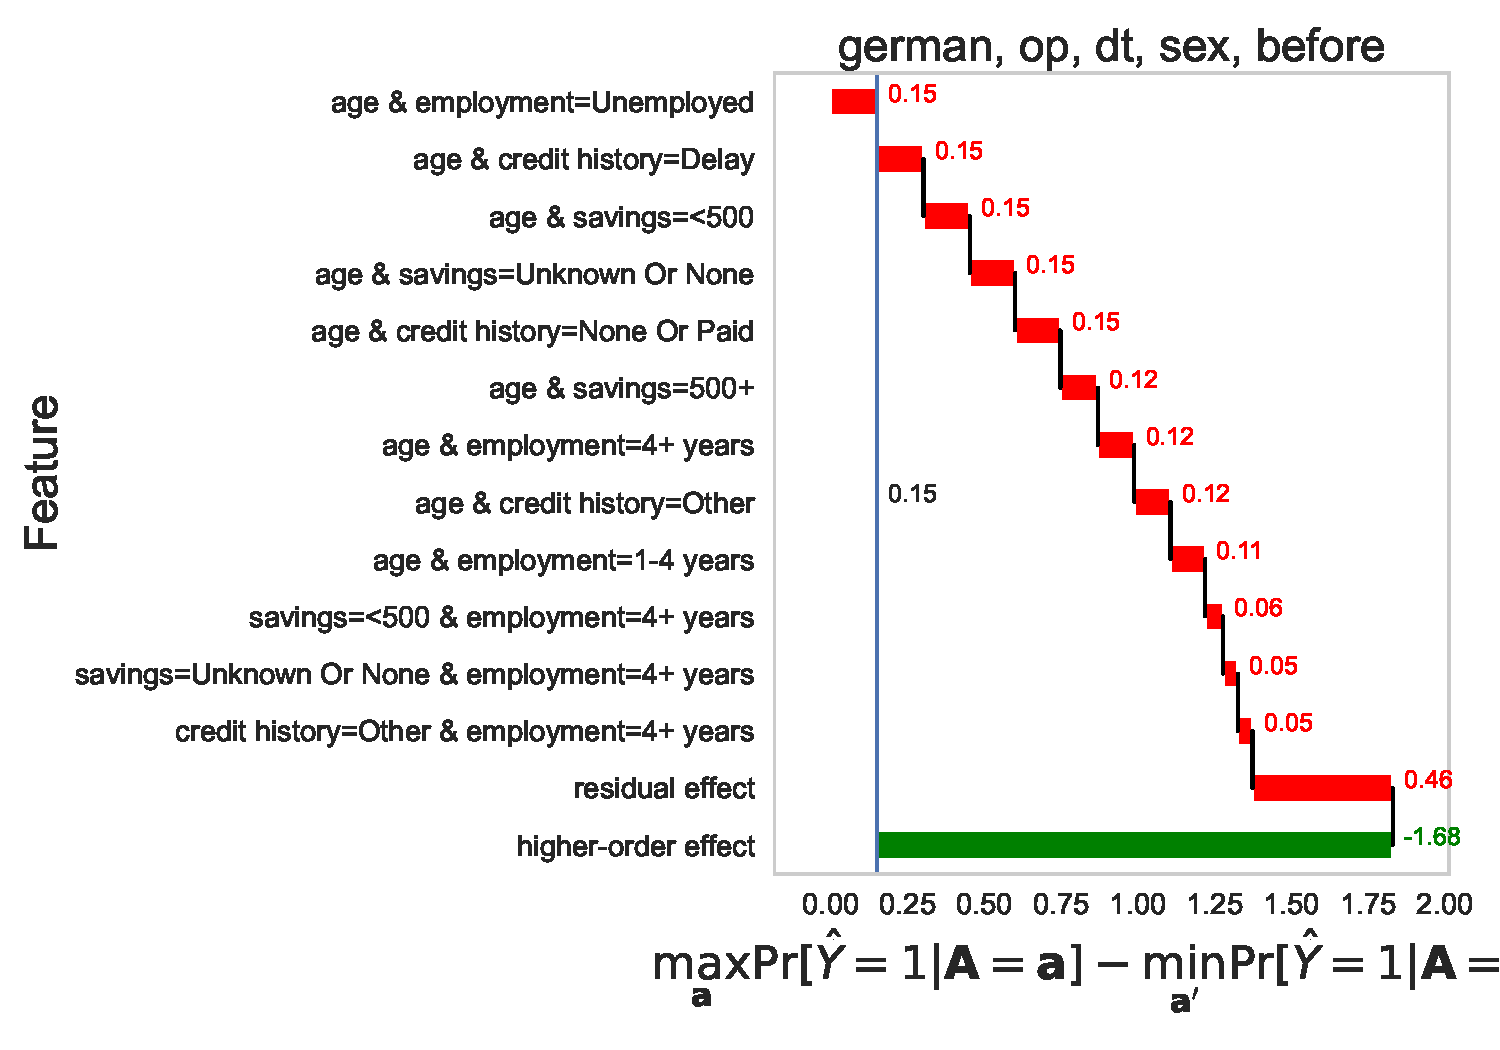
\includegraphics[scale=0.45]{figures/german_op_dt_sex_before}}\\
	\subfloat{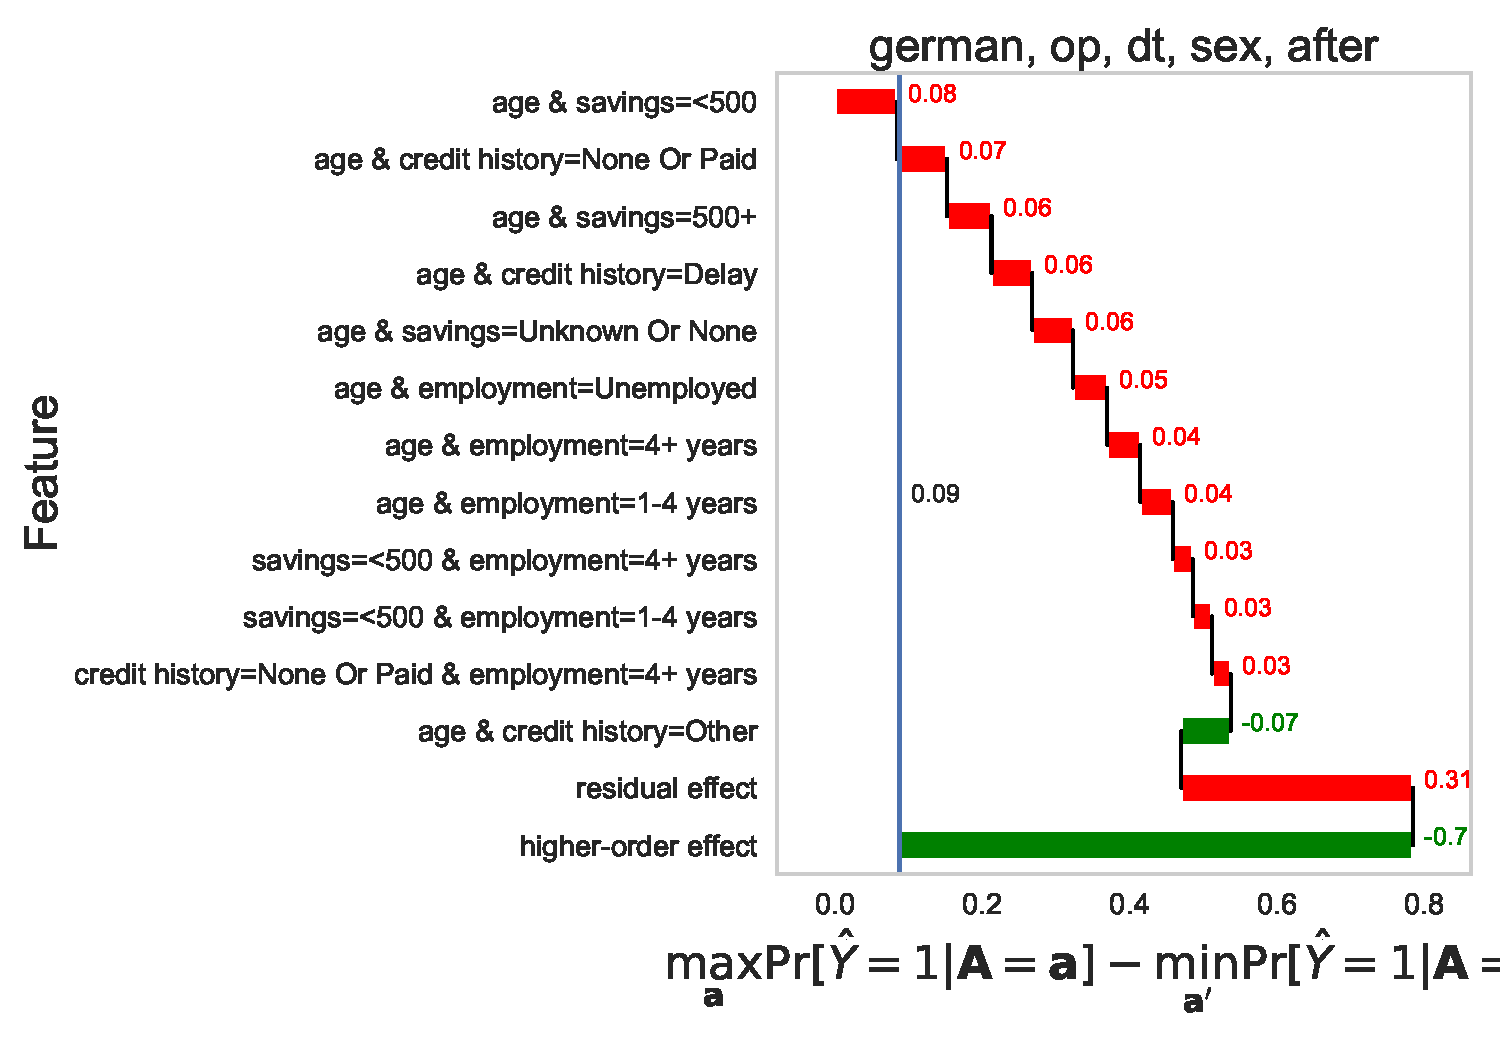
\includegraphics[scale=0.45]{figures/german_op_dt_sex_after}}
	\caption{Fairness enhancing preprocessing algorithm, optimized preprocessing. f\red{X axis should have the same X limit}}
\end{figure}


\begin{figure}
	\centering
	\subfloat{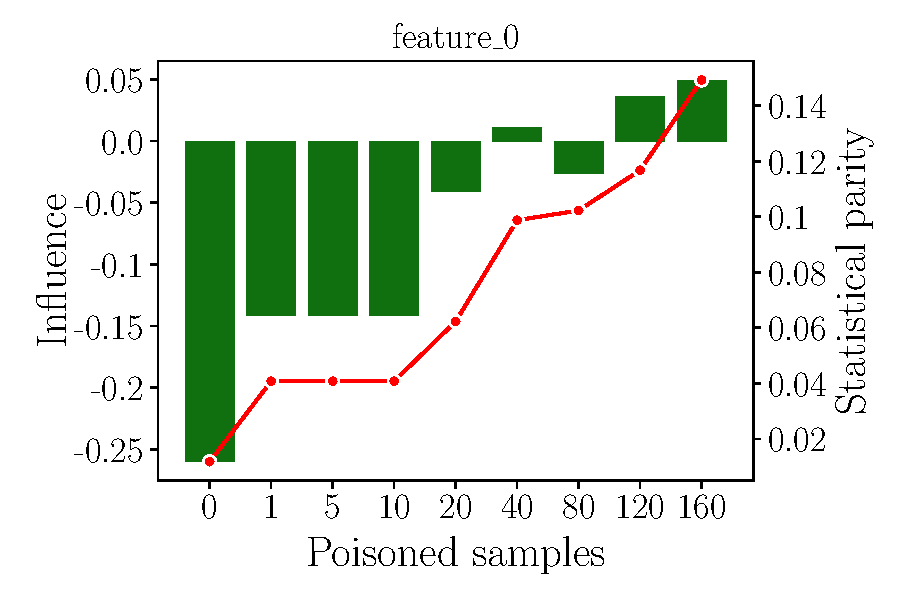
\includegraphics[scale=0.45]{figures/fairness_attack_feature_0}}
	\subfloat{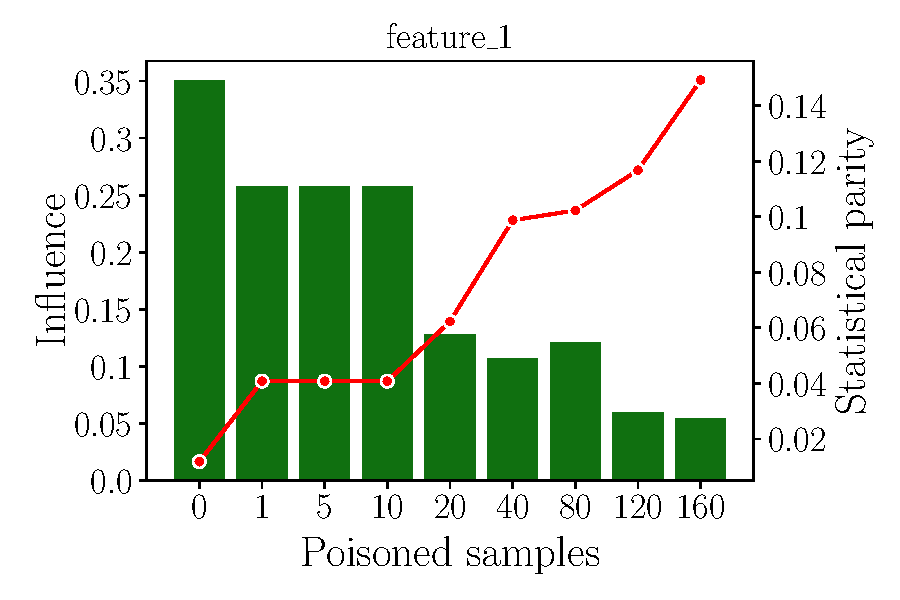
\includegraphics[scale=0.45]{figures/fairness_attack_feature_1}}\\
	\subfloat{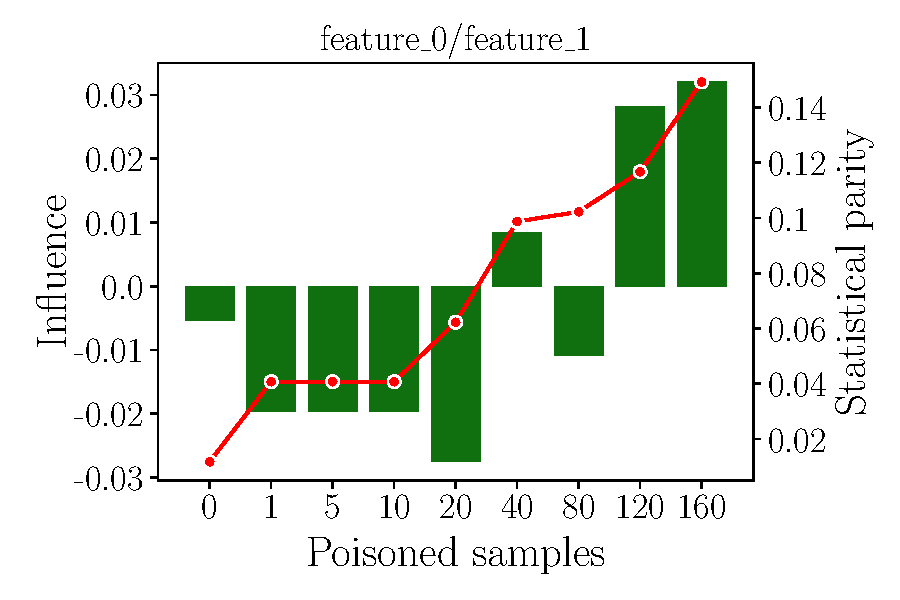
\includegraphics[scale=0.45]{figures/fairness_attack_feature_0_and_feature_1}}
	\subfloat{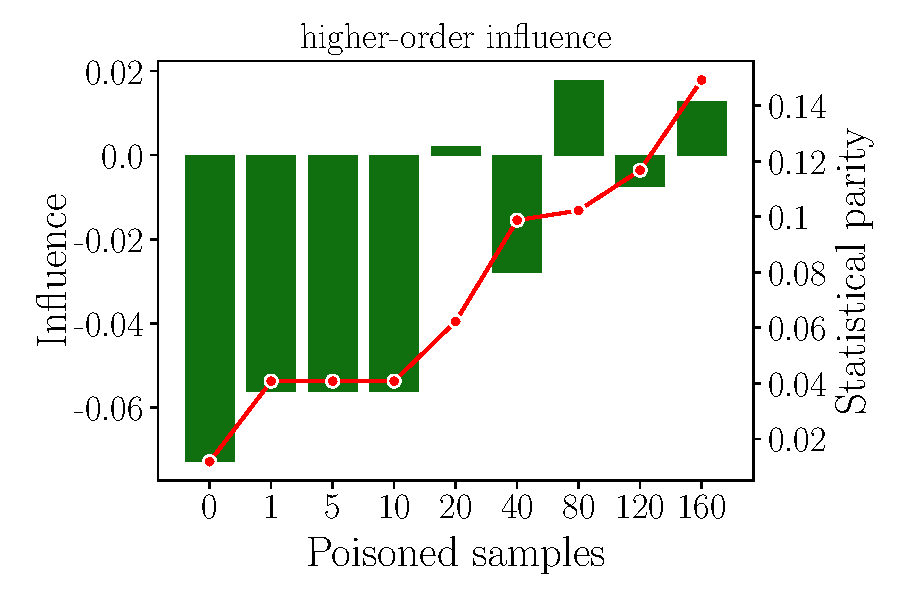
\includegraphics[scale=0.45]{figures/fairness_attack_higher-order_influence}}\\
	\caption{Fairness attack. Fairness influence is presented  in bar while statistical parity is shown in a line.}
\end{figure}


